\section{Reflections} \label{chap_reflection}

This section will dive into my enriching experiences and invaluable learnings acquired
while working on this research and thesis and is inspired by one of the master classes
about the \gls{ee} discipline. \gls{ee} encourages using grounded methodologies and
theories, like Five Way Framework, to comprehend the inner workings of an enterprise
\parencite{dietz_enterprise_2020}. I will apply the so-called Five Way Framework to
reflect on this research. By incorporating the Five Way Framework into the section, I
aspire to coherently showcase my learnings and reflections, shedding light on my thought
processes, strategies, modeling techniques, working methodologies, and support mechanisms.

\begin{figure}[H]
    \centering
    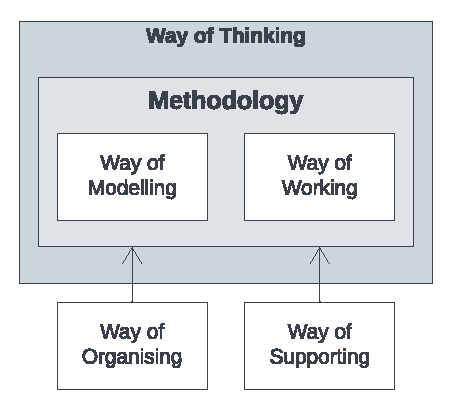
\includegraphics[width=0.5\textwidth]{figures/5ways.pdf}
    \caption[The Five Way Framework]{The Five Way Framework, inspired by \textcite{dietz_enterprise_2020}}
    \label{fig_5ways}
\end{figure}

\subsection{Way of Thinking}

Early in my career, I became obsessed with Software Quality and Maintainability. The
\gls{ns} theory shifted the obsession toward Stability and Evolvability. Gaining a
thorough understanding of the essential principles of this theory has boosted my
confidence in making informed decisions regarding all aspects of architecture, not just
limited to software.

As a Domain Architect, my job involved creating software products using the \gls{mdd}
paradigm. Initially, I was skeptical about this approach based on my early experiences.
The theory of \gls{ns} taught me to understand better the reasoning and characteristics of
code generation, on which I then realized that my skepticism was more about the process
caused as an effect on the implementation of the \gls{mdd}. The knowledge of \gls{ns}
helped me gain a clearer vision and helped me push the roadmap on the \gls{mdd} framework
in the right direction.

\subsection{Way of Managing}

I should have been able to finish sooner. I was one of the first with a research topic and
started working on my artifact in the first month when starting this journey. The artifact
was as good as ready before the summer holidays of the first year. Unfortunately, I
postponed writing the thesis until a later moment. I want to think that next time I will
start sooner, but knowing myself, I need some pressure to perform the less fun tasks, like
writing this thesis.

The review process seemed difficult and sometimes even problematic for a couple of
reasons. Next time I will ensure having the proper tools and agree on procedures to
improve reviews from multiple proofreaders. Secondly, I noticed that having multiple
proofreaders sometimes steers in opposite directions. This sometimes affected my ability
to make decisions and negatively affected my confidence. Having a joined review document,
where all proofreaders can leave comments, will significantly improve this experience for
me and my proofreaders. Then there is the personal aspect of sometimes taking things too
personally, grounded in a lack of self-confidence. However, this experience improved my
self-confidence. 

\subsection{Way of Modeling}

To explain the implementation concepts of the artifact, I looked into various modeling
languages. Archimate was the first option I considered. However, during one of the \gls{ee}
masterclasses, I learned the hard way that Archimate is not always the best choice for
communicating your models to a broad audience. I thought about using basic "boxes and
arrows" but decided to use the UML2 standard because it is a formal modeling language.

\subsection{Way of Working}

I very much enjoyed designing and creating the C\# artifacts. In hindsight, I enjoyed it
so much that I put in way too much effort than was needed. I was very curious about the
aspects of code generation, the effect of code generation on stable and evolvable
artifacts, and meta-circularity characteristics. I am confident I could have arrived at
the same conclusions presented in this thesis using a manually built Restful C\# artifact.
However, the insights I gained on the subjects of code expansion are of invaluable value
to me. Therefore, I am very pleased and satisfied that I took the effort to build the Code
Expander as a primary artifact. 

The \gls{ns} theorems are formulated very clearly and abstractly, making them also
applicable outside the software engineering field. During the masterclasses, we learned
about the application of \gls{ns} in the domains of Firewalls, Document management
systems, and Evolvable Business Processes. I also experienced benefits in structuring and
maintaining my Thesis document using \gls{vscode} and Latex by applying the principle of
\gls{soc} in managing the various chapters and sections. 

\subsection{Way of Supporting}

At the beginning of my research, I received a thorough introduction to the \gls{ns}
Theories and the Prime Radiant tooling from an employer at NSX. This introduction was
extremely helpful in gaining a better understanding of the fundamentals of \gls{ns}. It
also inspired me to consider the Code Expansion as a primary artifact. 

For the writing of the Thesis, I decided to use Latex. I quickly discovered that Overleaf
was one of the most popular editors. Nevertheless, I continued my search since I rejected
the idea of relying on online tooling for writing my Thesis. At some point, I decided to
experiment with my favorite code editor \gls{vscode}, and with the help of a latex package
manager and some \gls{vscode} plugins, I was able to create a fully-fledged Latex Editor
in \gls{vscode}, being able to use all the other benefits that come with \gls{vscode}. In
my next project, I will likely use the \gls{vscode} Latex editor again.
